\documentclass[a4paper, 11pt,oneside,openany, danish]{memoir} % Starter dokumentet af klassen memoir


%%%%%%%%%%%%%%%%%%%%%%%
		       % PREAMBLE %			
%%%%%%%%%%%%%%%%%%%%%%%



% Papirstørrelse og margener
\usepackage[paper=a4paper, hmargin=1.1in, vmargin=1.1in]{geometry}

% Font encoding og sprog
\usepackage[T1]{fontenc}					% Output encoding
\usepackage[utf8]{inputenc}				% Input encoding
\usepackage[danish]{babel}				% Sprog (orddeling)
\renewcommand{\danishhyphenmins}{22} 	% bedre orddeling, minimum to tegn før og efter deling
\usepackage{lmodern}  					% gør underscores pænere
\usepackage{microtype} 					% laver micro ændringer i text for at udgå luft og orddeling


%% Forside text
%\usepackage{soul} % lege lege
%\sodef\an{}{0.2em}{.9em plus.6em}{1em plus.1em minus.1em}
%\newcommand\stext[1]{\an{\scshape#1}}

% Fyldetekst (Lorem ipsum)
\usepackage{blindtext}

% Tabeller
\usepackage{booktabs}
\usepackage{threeparttable}
\usepackage[tableposition=top]{caption}
\usepackage{tabularx}
\newcolumntype{C}{>{\let\newline\\\arraybackslash\hspace{0pt}}X}

%matematik
\usepackage{amsmath,amssymb,mathtools,bm}
\newcommand{\tsub}[1]{_{\textup{#1}}}
\def\doubleunderline#1{\underline{\underline{#1}}}
\usepackage[separate-uncertainty = true,multi-part-units=single]{siunitx}

% XColor: Farver
\usepackage[svgnames,dvipsnames,x11names]{xcolor}

% Figurer og floats
\usepackage[]{graphicx}
\graphicspath{{figurer/}}
\usepackage{placeins}
\usepackage{float}			% Muliggoer eksakt placering af floats, f.eks. \begin{figure}[H]

%%% Tegning af kasser
%\usepackage{calc,graphicx,color}
%\definecolor{mygreen}{rgb}{0,0.6,0}
%\definecolor{mygray}{rgb}{0.5,0.5,0.5}

% Biblatex til referencer
\usepackage[backend=bibtex]{biblatex}
\addbibresource{bibfil.bib}





% Hyper ref
\usepackage[ unicode=true, colorlinks=false, linktocpage=true, 
pdfborder={0 0 0}, pdfstartpage=1, pdfstartview=FitV, breaklinks=true,
pdfpagemode=UseNone, pageanchor=true, pdfpagemode=UseOutlines,
plainpages=false, bookmarksnumbered, bookmarksopen=true,
bookmarksopenlevel=1, hypertexnames=true, pdfhighlight=/O, urlcolor=Black,
linkcolor=Black, citecolor=Black]{hyperref}

% Clever ref
\usepackage{cleveref}



\settocdepth{subsection}
\setsecnumdepth{subsection}

% Sidetal
% Sidetal
\let\footruleskip\undefined
\usepackage{fancyhdr}
\usepackage{lastpage}
\pagestyle{fancy} 
\fancyhf{} 

\fancyhead[R]{\leftmark}
\fancyfoot[R]{\thepage \hspace{0.008in} af \pageref{LastPage}}

\fancypagestyle{}{
	\renewcommand{\headrulewidth}{0pt}
	\fancyhf{}
	\fancyfoot[R]{\thepage \hspace{0.008in} af \pageref{LastPage}}%
	
}


% Starten på dokumentet
\begin{document}


%%%%%%%%%%%%%%%%%%%%%%%
		       % FORSIDEN %			
%%%%%%%%%%%%%%%%%%%%%%%

% !TEX root = ../prj4projektdokumentation.tex
% SKAL STÅ I TOPPEN AF ALLE FILER FOR AT MASTER-filen KOMPILERES 
\thispagestyle{empty}
{\centering
	{\scshape\LARGE Aarhus Universitet \par}
	\vspace{1cm}
	{\scshape\Large 4. semesterprojekt gruppe 1\par}
	{\scshape\Large Projektdokumentation\par}
	\vspace{1.5cm}
	{\huge\bfseries Spændingsregulator\par}
	\vspace{2cm}
	{\Large
		201509249 - Caroline Møller Sørensen\\
		201611140 - Sophia Amailie Mortensen\\
		201505195 - Dennis Slot Larsen \\
		201505115 - Laurids Givskov Jørgensen\\
		201508333 - Søren Jensen\\
		13114 - Jeppe Hansen\\  }
	\vfill
	Vejleder\par
	Emir Pasic
	
	\vfill
	
	{\large \today\par}
	\par}




\frontmatter
%%%%%%%%%%%%%%%%%%%%%%%
             % RESUME & ABSTRACT %			
%%%%%%%%%%%%%%%%%%%%%%%



%%%%%%%%%%%%%%%%%%%%%%%
         % INDHOLDSFORTEGNELSE %			
%%%%%%%%%%%%%%%%%%%%%%%

\tableofcontents

%%%%%%%%%%%%%%%%%%%%%%%
                        % KAPITLER %			
%%%%%%%%%%%%%%%%%%%%%%%

\mainmatter
% !TEX root = ../prj4projektdokumentation.tex
% SKAL STÅ I TOPPEN AF ALLE FILER FOR AT MASTER-filen KOMPILERES 

\chapter{Introduktion}

\section{Problemformulering}
Når belastningerne i et distributionssystem ændres, vil spændingsniveauet variere. Det er vigtigt, at spændingsniveauet holdes stabilt. Hvordan sikres dette?
% !TEX root = ../prj4projektdokumentation.tex
% SKAL STÅ I TOPPEN AF ALLE FILER FOR AT MASTER-filen KOMPILERES 

\chapter{Projektbeskrivelse}

Formålet med dette projekt, er at opbygge et system, der simulerer det danske transmissionssystem. For energileverandører i Danmark er det et lovmæssigt krav, at spændingsforsyningen hos forbrugerne altid ligger på $\pm$ 230 volt, og det ønskes at undersøge mulighederne for at opfylde dette.\\ 
I dette projekt vil fokus være på stykket fra distributionstransformer og ud til forbrugere/belastninger. Systemet skal bestå af en spændingsregulator (trinkobler), en distributionslinje og to eller flere varierende belastninger. Det ønskes at måle strøm, spænding, power factor og effektretning således, at spændingsregulatoren hele tiden kan holde spændingen på $\pm$ et givent niveau, selvom belastningen ændres. Normalt måles disse værdier ved distributionstransformeren, men i dette projekt ønskes det at måle hos hver enkelt belastning. På den måde fås en bedre overvågning af systemet og bedre mulighed for at observere hvilken betydning, f.eks. belastningens afstand til distributionstransformeren har for spændingsniveauet.\\ Systemet skal have to indstillinger – en til manuelt valg af spændingsniveau og en til automatisk valg af passende spændingsniveau.\\ 
Det ønskes desuden at kunne måle frekvensindholdet i systemet for at kunne observere et eventuelt indhold af harmoniske. De harmoniske i systemet er højfrekvente og vil afsætte varme i transformerne og dermed forkorte deres levetid. Det er derfor relevant at kende til indholdet af disse.\\ 
Det er et krav, at målte værdier i systemet vises på en skærm. 

\begin{figure}[htbp] % (alternativt [H])
	\centering
	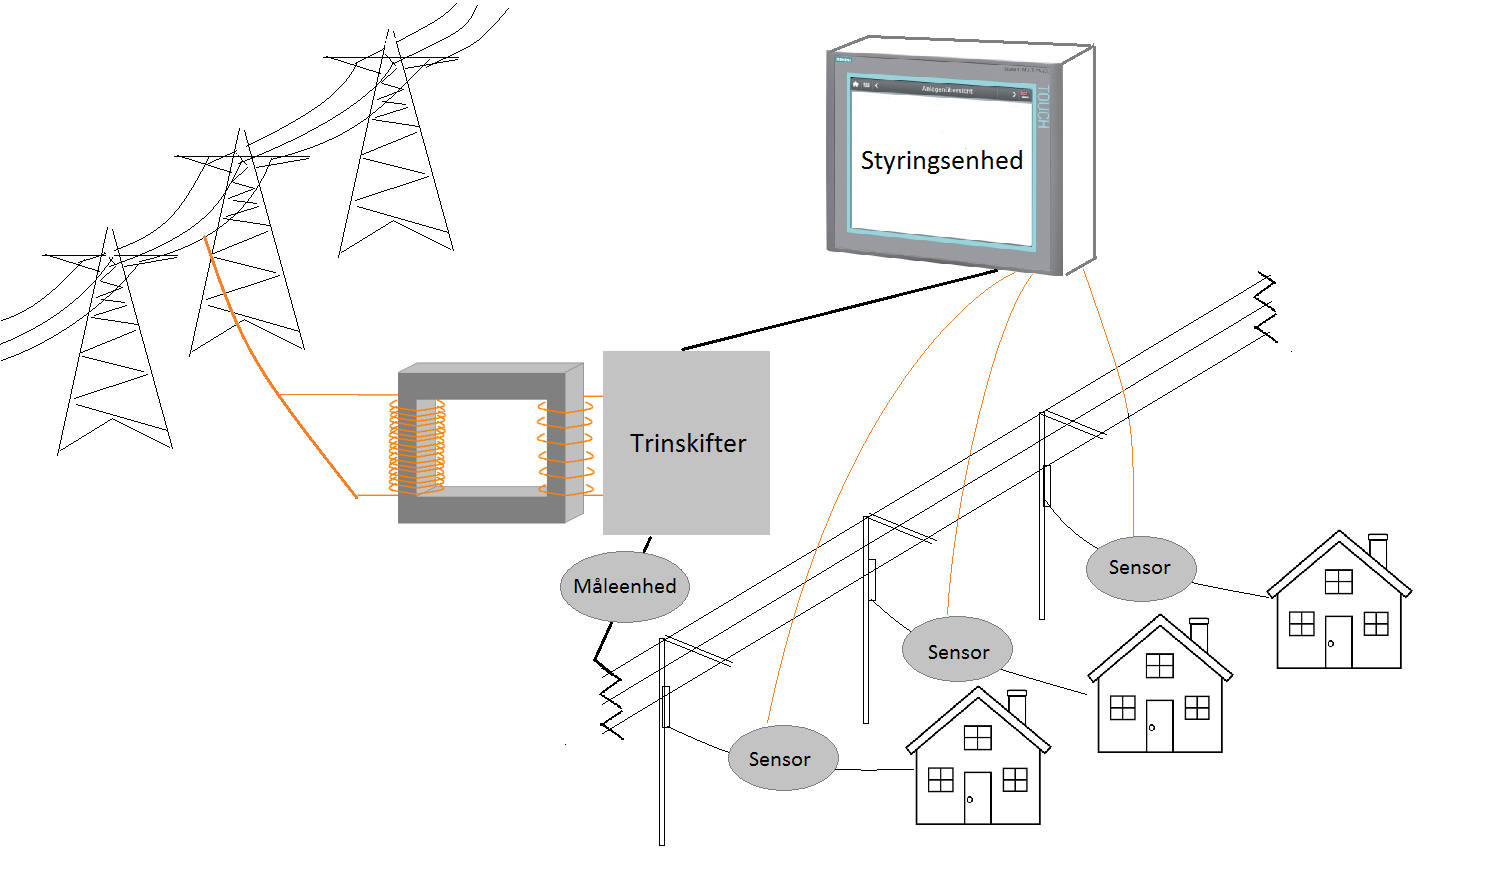
\includegraphics[width=0.7\textwidth]{Figure/RigtBillede}
	\caption{Visuel fremvisning af system}
	\label{fig:Rigtbillede}
\end{figure}
% !TEX root = ../prj4projektdokumentation.tex
% SKAL STÅ I TOPPEN AF ALLE FILER FOR AT MASTER-filen KOMPILERES 
\chapter{Kravspecifikation}
% !TEX root = ../../prj4projektdokumentation.tex
% SKAL STÅ I TOPPEN AF ALLE FILER FOR AT MASTER-filen KOMPILERES 

\section{Systembeskrivelse}

Systemet der er udviklet har til opgave at regulere spændingsniveauet på en distributionslinje, afhængigt af målingerne fra sensorer ved hver forbruger.
I dette projekt er det ikke muligt at realisere, derfor udvikles et produkt, der kan simulere scenariet. Det simuleres ved at skalere spændingsniveauet fra standardniveauet på 230V ned til 4V på distributionssiden. Dette gør det muligt at arbejde med en 8-trins transformer med specifikationen 24V/8-0V.\\
I prototypen er udviklet en impedans til simulering af en distributionslinje med en længde svarende til en typisk distributionslinje.\\
På distributionslinjen er så placeret et antal belastninger, der skal illustrere en husstand. Disse er designet således, at skalering passer med resten af systemet. Dette er rammen systemet skal arbejde indenfor. \\
To typer måleenheder er fremstillet; en placeret centralt på sekundær side af transformeren, og en som er placeret ved hver belastning. De decentrale måleenheder kan måle spænding, strøm og faseforskydning. Den centrale måleenhed kan også måle indeholdet af harmoniske frekvenser. Systemets frekvens er 50Hz ligesom frekvensen på det danske elnet.\\
Data fra måleenhederne samles så i en styringsenhed, der har til opgave at regulere spændingsniveauet, så det altid ligger på 4V på distributionssiden ved at skifte trin på transformeren. Selve trinskiftet står trinskiftenheden for.\\
På styringsenheden er det muligt at observere de målte værdier på en touchskærm. Ved manuel styring er det på samme touchskærm, der kan skiftes trin på transformeren.\\
Systemet, der er fremstillet, er en simulering af et produkt, der kan løse problemformuleringen. Den overordnet struktur er dog tænkt sådan, at den kan skaleres op.\\




\subsection{Termliste}

\begin{table}[htbp]
\centering
\begin{tabular}{|l|l|}
\hline
\textbf{Term} 	& \textbf{Beskrivelse} \\\hline
Spændingsregaulator	& Består af en transformer og tilkoblet sensorer \\\hline
Trin 	& Trin af spændingsniveau \\\hline

\end{tabular}
\caption{Termbeskrivelse}
\label{tab:termbeskrivelsen}

\end{table}
% !TEX root = ../../prj4projektdokumentation.tex
% SKAL STÅ I TOPPEN AF ALLE FILER FOR AT MASTER-filen KOMPILERES 

\section{MoSCoW}

\begin{itemize}
\item{Systemet skal bestå af en trin transformator 230/20V der skifter mellem tre trin (??)}
\item{Systemet skal måle spændingen, strømmen, effektretning og power factor}
\item{Systemet skal vise data på skærm/brugergrænseflade}
\item{Systemet skal simulere en distributionslinje og belastning}
\item{Systemet skal bestå af en manuel spændingsregulering}
\item{Systemet skal kunne måle harmoniske}
\item{Systemet burde bestå af en automatisk spændingsregulering}
\item{Systemet kunne have en log}
\item{Systemet kunne have flere belastninger}
\item{Distributionslinjen kunne indeholde en decentral producent, som giver anledning til overspændinger på nettet}
\item{Systemet vil ikke kunne fjerne harmoniske} 
\end{itemize}


% !TEX root = ../../prj4projektdokumentation.tex
% SKAL STÅ I TOPPEN AF ALLE FILER FOR AT MASTER-filen KOMPILERES 

\section{Funktionelle krav}
I dette afsnit beskrives de funktionelle krav for systemet. De dele, hvor en bruger interager med systemet er beskrevet med usecase diagrammer. Den automatiske del er beskrevet og vist vha. et STM diagram.

\subsection{Beskrivelse af automatisk mode}
\label{Afsnit: Automatisk mode}

Når spændingsregulatoren er i automatisk mode, kontrolleres spænding ved forbrugerne. Hvis den spænding er for høj eller lav iht. de 4V skiftes der et trin op eller et trin ned.  
\begin{figure}[htbp] % (alternativt [H])
	\centering
	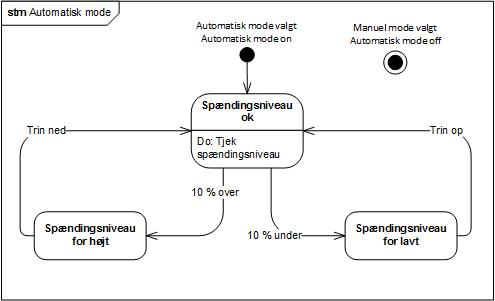
\includegraphics[width=0.8\textwidth]{Figure/STM}
	\caption{Beskrivelse af automatisk mode}
	\label{fig:automode}
\end{figure}

\subsection{Usecase Diagram}

\begin{figure}[H] % (alternativt [H])
	\centering
	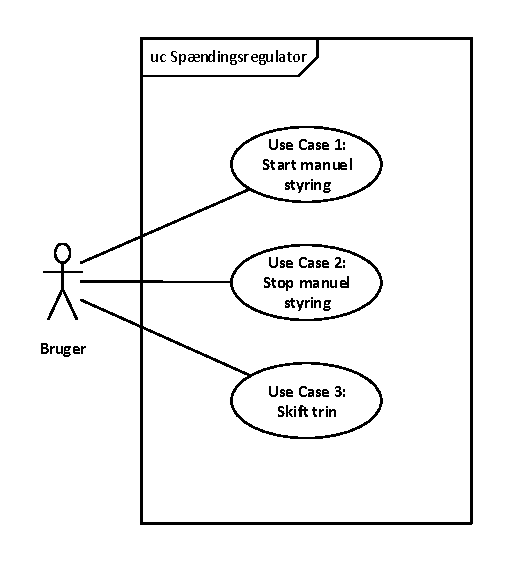
\includegraphics[width=0.5\textwidth]{Figure/UsecaseDiagram}
	\caption{Usecase Diagram}
	\label{fig:UsecaseDiagram}
\end{figure}
Systemet indholder tre usecases, der alle er initieret af brugeren. Den automatiske del af systemet er beskrevet i afsnit \ref{Afsnit: Automatisk mode}.

\subsection{Aktør Beskrivelse}
\textbf{Brugeren} er den primær aktør. En sikkerhedsgodkendt operatør der kan betjene systemet.

\subsection{Usecase 1 - Start manuel styring}
\begin{table}[H]
	\centering
	
	\begin{threeparttable}
		\begin{tabularx}{\linewidth}{ l X }
			\toprule
			\bfseries{Navn:}				& UC1 - Start manuel styring  \\
			\midrule
			\bfseries{Mål:} 				& At sætte systemet i manuel mode \\
			\midrule
			\bfseries{Initiering:} 			& Initieres af brugeren. \\
			\midrule
			\bfseries{Aktører:} 			& Brugeren (Primær) \\
			\midrule
			\bfseries{Samtidige forekomster:} & 1 \\
			\midrule
			\bfseries{Forudsætninger:} 		& At systemet er funktionelt og i automatisk mode\\
			\midrule
			\bfseries{Resultat:} 			& Systemet er i manuel mode \\
			\midrule
			\bfseries{Hovedscenariet:} 	& \\
			
			
			1 	& Brugeren trykker Manuel styring på skærmen.\\
			2	& Systemet skifter til Manuel mode. \\
			3 	& Systemet aktivere manuel skærm. 	\\
			
			\bottomrule
			
		\end{tabularx}
	\end{threeparttable}
	\caption{Fully dressed use case for UC1 - Start manuel styring}
	\label{table:UC1}
\end{table}

\subsection{Usecase 2 - Stop manuel styring}

\begin{table}[H]
	\centering
	
	\begin{threeparttable}
		\begin{tabularx}{\linewidth}{ l X }
			\toprule
			\bfseries{Navn:}				& UC2 - Stop manuel styring  \\
			\midrule
			\bfseries{Mål:} 				& At sætte systemet i automatisk mode \\
			\midrule
			\bfseries{Initiering:} 			& Initieres af brugeren. \\
			\midrule
			\bfseries{Aktører:} 			& Brugeren (Primær) \\
			\midrule
			\bfseries{Samtidige forekomster:} & 1 \\
			\midrule
			\bfseries{Forudsætninger:} 		& At systemet er funktionelt og i manuel mode\\
			\midrule
			\bfseries{Resultat:} 			& Systemet er i automatisk mode \\
			\midrule
			\bfseries{Hovedscenariet:} 	& \\
			
			
			1 	& Brugeren trykker Automatisk styring på skærmen.\\
			2 	& Systemet skifter til Automatisk mode.\\
			3 	& Systemet aktivere automatisk skærm. 	\\		
				
			
			\bottomrule
			
		\end{tabularx}
	\end{threeparttable}
	\caption{Fully dressed use case for UC2 - Stop manuel styring}
	\label{table:UC2}
\end{table}

\subsection{Usecase 3a - Skift trin}

\begin{table}[H]
	\centering
	
	\begin{threeparttable}
		\begin{tabularx}{\linewidth}{ l X }
			\toprule
			\bfseries{Navn:}				& UC3a - Skift trin op  \\
			\midrule
			\bfseries{Mål:} 				& At skifte et trin op på transformeren \\
			\midrule
			\bfseries{Initiering:} 			& Initieres af brugeren. \\
			\midrule
			\bfseries{Aktører:} 			& Brugeren (Primær) \\
			\midrule
			\bfseries{Samtidige forekomster:} & 1 \\
			\midrule
			\bfseries{Forudsætninger:} 		& At systemet er funktionelt og i manuel mode\\
			\midrule
			\bfseries{Resultat:} 			& Transformerens trin er skiftet et trin op \\
			\midrule
			\bfseries{Hovedscenariet:} 	& \\
			
			
			1 	& Brugeren vælger Trin Op på skærmen.\\
			2 	& Systemet skifter et trin op på transformeren.\\
			3 	& Aktuelt trin vises på skærmen.\\
			4 	& Måleværdier opdateres på skærmen.\\		
			
			\bottomrule
			
		\end{tabularx}
	\end{threeparttable}
	\caption{Fully dressed use case for UC3 - Skift trin}
	\label{table:UC3}
\end{table}

\subsection{Usecase 3b - Skift trin}

\begin{table}[H]
	\centering
	
	\begin{threeparttable}
		\begin{tabularx}{\linewidth}{ l X }
			\toprule
			\bfseries{Navn:}				& UC3b - Skift trin ned  \\
			\midrule
			\bfseries{Mål:} 				& At skifte et trin ned på transformeren \\
			\midrule
			\bfseries{Initiering:} 			& Initieres af brugeren. \\
			\midrule
			\bfseries{Aktører:} 			& Brugeren (Primær) \\
			\midrule
			\bfseries{Samtidige forekomster:} & 1 \\
			\midrule
			\bfseries{Forudsætninger:} 		& At systemet er funktionelt og i manuel mode\\
			\midrule
			\bfseries{Resultat:} 			& Transformerens trin er skiftet et trin ned \\
			\midrule
			\bfseries{Hovedscenariet:} 	& \\
			
			
			1 	& Brugeren vælger Trin Ned på skærmen.\\
			2 	& Systemet skifter et trin ned på transformeren.\\
			3 	& Aktuelt trin vises på skærmen.\\
			4 	& Måleværdier opdateres på skærmen.\\			
			
			\bottomrule
			
		\end{tabularx}
	\end{threeparttable}
	\caption{Fully dressed use case for UC3 - Skift trin}
	\label{table:UC3}
\end{table}



% !TEX root = ../../prj4projektdokumentation.tex
\section{Ikke funktionelle krav}
% for spændingsregulator
\begin{table}[H]
	\centering
	\begin{tabular}{|p{4cm}|p{3cm}|p{3cm}|p{3cm}|p{1cm}|}
		\hline
		\textbf{Trintransformer} & \textbf{Handling} & \textbf{Forventet resultat} & \textbf{Resultat} &\textbf{OK} \\\hline
		Nominel spænding på primærsiden er 24VAC & Spændingen på primærsiden måles. & Den målte værdi er 24VAC. &  &  \\\hline
		Nominel spænding på sekundær side er 4, 5 eller 6 VAC afhængig af trin & Spændingen på sekundærsiden måles for hhv. trin 4, 5 og 6. & De målte værdier er 4, 5 og 6V &  & \\\hline
		Skal minimum kunne levere 500mA	. & Strømmen på sekundærsiden måles. & Transformerne kan levere over 500mA &   & \\\hline
	\end{tabular}
	
\end{table} 

% for belastning
\begin{table}[H]
	\centering
	\begin{tabular}{|p{4cm}|p{3cm}|p{3cm}|p{3cm}|p{1cm}|}
		\hline
		\textbf{Belastning} & \textbf{Handling} & \textbf{Forventet resultat} & \textbf{Resultat} &\textbf{OK} \\\hline
		Modstandsværdi på 54$\Omega$ giver spændingsfald på 10\%, når spændingen fra regulatoren er 4V. & Den givne modstand indsættes som belastning, og spændingen herover måles. & Spændingen over belastningen måles til 3,6V. &  &  \\\hline	
	\end{tabular}

	
\end{table}

% for måleenhed
%\begin{table}[htbp]
%	\centering
	\begin{longtable}{|p{4cm}|p{3cm}|p{3cm}|p{3cm}|p{1cm}|}
		\hline
		\textbf{Måleenhed} & \textbf{Handling} & \textbf{Forventet resultat} & \textbf{Resultat} &\textbf{OK} \\\hline
		Måle spændingen ved trinskifteren og forbrugerne mellem 0 og 8 Vrms & Måleenheden testes med spændinger fra 0 til 8Vrms, i intervaller af 500mV. & Korrekt spændingsmåling i hele intervallet. & & \\\hline
		Måle spændingen med en præcision på $\pm$ 5\%& Måleenheden påtrykkes en spænding på 3,5Vrms. Der laves herefter ti målinger& Gennemsnits afvigelsen forventes at være under $\pm$5\%.&  & \\\hline
		Måle strømmen ved trinskifteren og forbrugerne mellem 0 og 500mA& Måleenheden testes med strømme fra 0 til 500mA i intervaller af 50mA&Korrekt strømmåling i hele intervallet.& & \\\hline
		Måle strømmen med en præcision på $\pm$ 5\%&Måleenheden påtrykkes en spænding på 300mVrms (Svarende til 300mA), der laves herefter ti målinger&Gennemsnits afvigelsen forventes at være under $\pm$5\%& & \\\hline
		Måle og beregne power factor med en præcision på $\pm$ 5$\%$&Måleenheden måler power factor over en belastning på distributionslinjen, der sammenlignes med beregnet power factor&Afvigelsen forventes at være under $\pm$ 5\% & & \\\hline
		Beregne THD med en præcision på $\pm$ 5$\%$&Måleenheden påtrykkes en firkantsignal med 1V amplituder og 1V offset. Der sammenlignes med beregnet THD for firkantsignal& Afvigelsen forventes at være under $\pm$ 5\%& & \\\hline
			
	\end{longtable}
	
	
%\end{table}
% !TEX root = ../prj4projektdokumentation.tex

\chapter{Accepttestspecifikation}


% !TEX root = ../../prj4projektdokumentation.tex
% SKAL STÅ I TOPPEN AF ALLE FILER FOR AT MASTER-filen KOMPILERES 

\section{Funktionelle krav}
I dette afsnit beskrives de funktionelle krav for systemet. De dele, hvor en bruger interager med systemet er beskrevet med usecase diagrammer. Den automatiske del er beskrevet og vist vha. et STM diagram.

\subsection{Beskrivelse af automatisk mode}
\label{Afsnit: Automatisk mode}

Når spændingsregulatoren er i automatisk mode, kontrolleres spænding ved forbrugerne. Hvis den spænding er for høj eller lav iht. de 4V skiftes der et trin op eller et trin ned.  
\begin{figure}[htbp] % (alternativt [H])
	\centering
	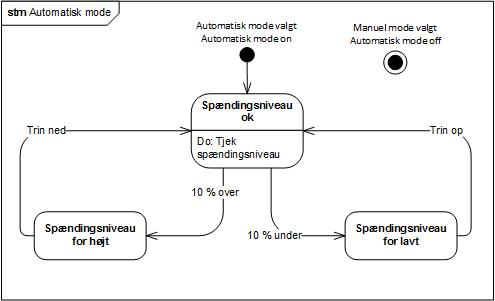
\includegraphics[width=0.8\textwidth]{Figure/STM}
	\caption{Beskrivelse af automatisk mode}
	\label{fig:automode}
\end{figure}

\subsection{Usecase Diagram}

\begin{figure}[H] % (alternativt [H])
	\centering
	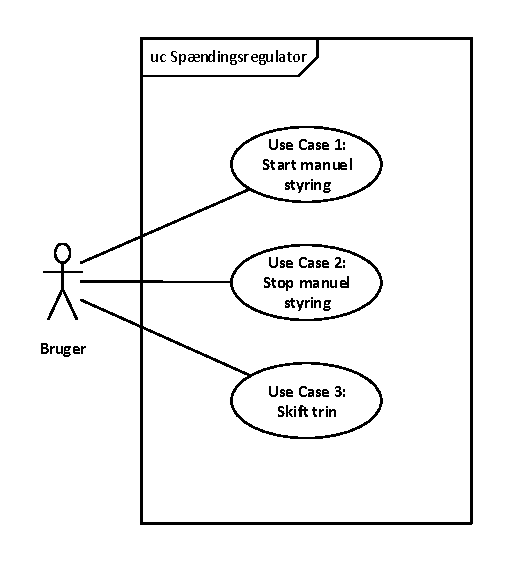
\includegraphics[width=0.5\textwidth]{Figure/UsecaseDiagram}
	\caption{Usecase Diagram}
	\label{fig:UsecaseDiagram}
\end{figure}
Systemet indholder tre usecases, der alle er initieret af brugeren. Den automatiske del af systemet er beskrevet i afsnit \ref{Afsnit: Automatisk mode}.

\subsection{Aktør Beskrivelse}
\textbf{Brugeren} er den primær aktør. En sikkerhedsgodkendt operatør der kan betjene systemet.

\subsection{Usecase 1 - Start manuel styring}
\begin{table}[H]
	\centering
	
	\begin{threeparttable}
		\begin{tabularx}{\linewidth}{ l X }
			\toprule
			\bfseries{Navn:}				& UC1 - Start manuel styring  \\
			\midrule
			\bfseries{Mål:} 				& At sætte systemet i manuel mode \\
			\midrule
			\bfseries{Initiering:} 			& Initieres af brugeren. \\
			\midrule
			\bfseries{Aktører:} 			& Brugeren (Primær) \\
			\midrule
			\bfseries{Samtidige forekomster:} & 1 \\
			\midrule
			\bfseries{Forudsætninger:} 		& At systemet er funktionelt og i automatisk mode\\
			\midrule
			\bfseries{Resultat:} 			& Systemet er i manuel mode \\
			\midrule
			\bfseries{Hovedscenariet:} 	& \\
			
			
			1 	& Brugeren trykker Manuel styring på skærmen.\\
			2	& Systemet skifter til Manuel mode. \\
			3 	& Systemet aktivere manuel skærm. 	\\
			
			\bottomrule
			
		\end{tabularx}
	\end{threeparttable}
	\caption{Fully dressed use case for UC1 - Start manuel styring}
	\label{table:UC1}
\end{table}

\subsection{Usecase 2 - Stop manuel styring}

\begin{table}[H]
	\centering
	
	\begin{threeparttable}
		\begin{tabularx}{\linewidth}{ l X }
			\toprule
			\bfseries{Navn:}				& UC2 - Stop manuel styring  \\
			\midrule
			\bfseries{Mål:} 				& At sætte systemet i automatisk mode \\
			\midrule
			\bfseries{Initiering:} 			& Initieres af brugeren. \\
			\midrule
			\bfseries{Aktører:} 			& Brugeren (Primær) \\
			\midrule
			\bfseries{Samtidige forekomster:} & 1 \\
			\midrule
			\bfseries{Forudsætninger:} 		& At systemet er funktionelt og i manuel mode\\
			\midrule
			\bfseries{Resultat:} 			& Systemet er i automatisk mode \\
			\midrule
			\bfseries{Hovedscenariet:} 	& \\
			
			
			1 	& Brugeren trykker Automatisk styring på skærmen.\\
			2 	& Systemet skifter til Automatisk mode.\\
			3 	& Systemet aktivere automatisk skærm. 	\\		
				
			
			\bottomrule
			
		\end{tabularx}
	\end{threeparttable}
	\caption{Fully dressed use case for UC2 - Stop manuel styring}
	\label{table:UC2}
\end{table}

\subsection{Usecase 3a - Skift trin}

\begin{table}[H]
	\centering
	
	\begin{threeparttable}
		\begin{tabularx}{\linewidth}{ l X }
			\toprule
			\bfseries{Navn:}				& UC3a - Skift trin op  \\
			\midrule
			\bfseries{Mål:} 				& At skifte et trin op på transformeren \\
			\midrule
			\bfseries{Initiering:} 			& Initieres af brugeren. \\
			\midrule
			\bfseries{Aktører:} 			& Brugeren (Primær) \\
			\midrule
			\bfseries{Samtidige forekomster:} & 1 \\
			\midrule
			\bfseries{Forudsætninger:} 		& At systemet er funktionelt og i manuel mode\\
			\midrule
			\bfseries{Resultat:} 			& Transformerens trin er skiftet et trin op \\
			\midrule
			\bfseries{Hovedscenariet:} 	& \\
			
			
			1 	& Brugeren vælger Trin Op på skærmen.\\
			2 	& Systemet skifter et trin op på transformeren.\\
			3 	& Aktuelt trin vises på skærmen.\\
			4 	& Måleværdier opdateres på skærmen.\\		
			
			\bottomrule
			
		\end{tabularx}
	\end{threeparttable}
	\caption{Fully dressed use case for UC3 - Skift trin}
	\label{table:UC3}
\end{table}

\subsection{Usecase 3b - Skift trin}

\begin{table}[H]
	\centering
	
	\begin{threeparttable}
		\begin{tabularx}{\linewidth}{ l X }
			\toprule
			\bfseries{Navn:}				& UC3b - Skift trin ned  \\
			\midrule
			\bfseries{Mål:} 				& At skifte et trin ned på transformeren \\
			\midrule
			\bfseries{Initiering:} 			& Initieres af brugeren. \\
			\midrule
			\bfseries{Aktører:} 			& Brugeren (Primær) \\
			\midrule
			\bfseries{Samtidige forekomster:} & 1 \\
			\midrule
			\bfseries{Forudsætninger:} 		& At systemet er funktionelt og i manuel mode\\
			\midrule
			\bfseries{Resultat:} 			& Transformerens trin er skiftet et trin ned \\
			\midrule
			\bfseries{Hovedscenariet:} 	& \\
			
			
			1 	& Brugeren vælger Trin Ned på skærmen.\\
			2 	& Systemet skifter et trin ned på transformeren.\\
			3 	& Aktuelt trin vises på skærmen.\\
			4 	& Måleværdier opdateres på skærmen.\\			
			
			\bottomrule
			
		\end{tabularx}
	\end{threeparttable}
	\caption{Fully dressed use case for UC3 - Skift trin}
	\label{table:UC3}
\end{table}



% !TEX root = ../../prj4projektdokumentation.tex
% SKAL STÅ I TOPPEN AF ALLE FILER FOR AT MASTER-filen KOMPILERES 

\chapter{Arkitektur}

% !TEX root = ../../prj4projektdokumentation.tex
% SKAL STÅ I TOPPEN AF ALLE FILER FOR AT MASTER-filen KOMPILERES 

\section{Blok definitionsdiagram}
Et BDD for spændingsregulator ses på figur \ref{fig:BDDSpaendingsregulator}. På diagrammet ses de overordnet blokke spædingsregulator består af. En beskrivelse af hver blok kan læses under figur \ref{fig:BDDSpaendingsregulator}.

\begin{figure}[htbp] % (alternativt [H])
	\centering
	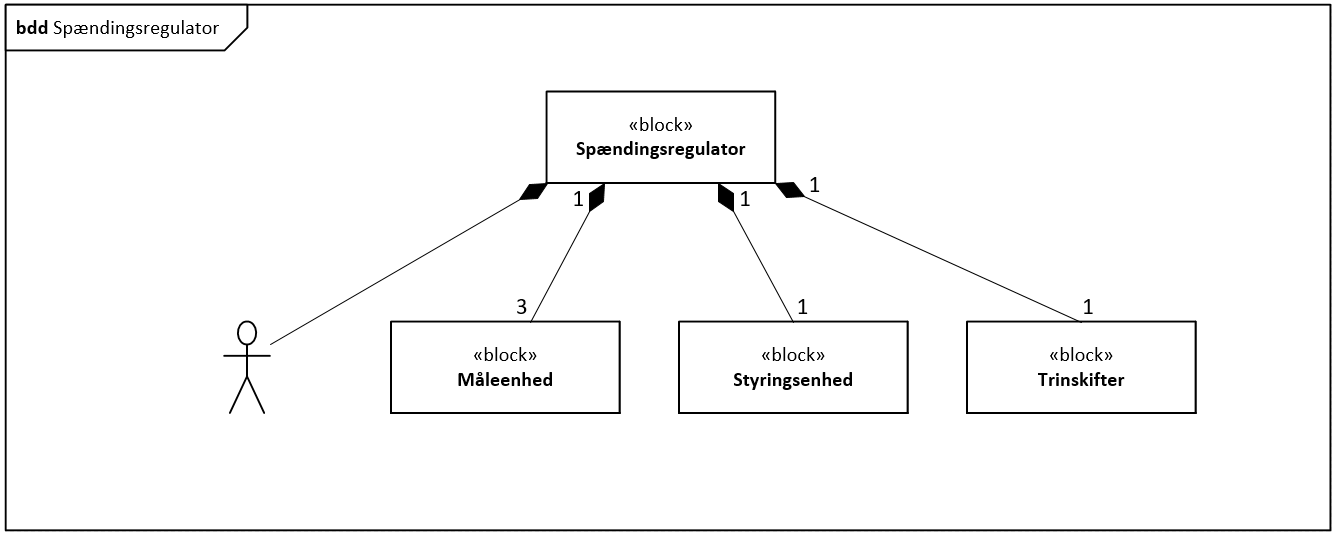
\includegraphics[width=0.9\textwidth]{Figure/BDDSpaendingsregulator}
	\caption{BDD Spændingsregulator}
	\label{fig:BDDSpaendingsregulator}
\end{figure}

\textbf{Måleenhed} står for at måle spænding, strøm og faseforskydningen herimellem. Ligeledes skal denne kunne måle indeholdet af harmoniske frekvenser. Den består af hardware til måling af de nævnte parametre og en PSoC 5. På enheden ligger også en del af behandlingen af rådataet, så dette kan formidles til styringsenheden.

\textbf{Styringsenhed} har til opgave at styre trinskifteren ud fra de data den får fra målenehderne. Den består af en PLC, tl styringen og et HMI, der skal give en bruger overblik over status for distributionslinjen.

\textbf{Trinskifter} er en enhed der kan skifte trin på transformeren ud fra et signal fra styringsenheden. Den består altå af en kontakt for hvert trin, der kan kontrolleres af styringsenheden.
% !TEX root = ../../prj4projektdokumentation.tex
% SKAL STÅ I TOPPEN AF ALLE FILER FOR AT MASTER-filen KOMPILERES 

\section{Intern blok diagram}
På figur \ref{fig:IBDSp} og figur \ref{fig:IBDSt} ses IBD for henholdsvis Spændingsregulator og Styringsenhed. På diagrammerne ses de interne forbindelser i systemet. Under figurne er tilhørende signalbeskrivelser, se tabel \ref{tab:SignalbeskrivelseSp} og tabel \ref{tab:SignalbeskrivelseSt}, der uddyber diagrammerne nærmere.

\begin{figure}[htbp] % (alternativt [H])
	\centering
	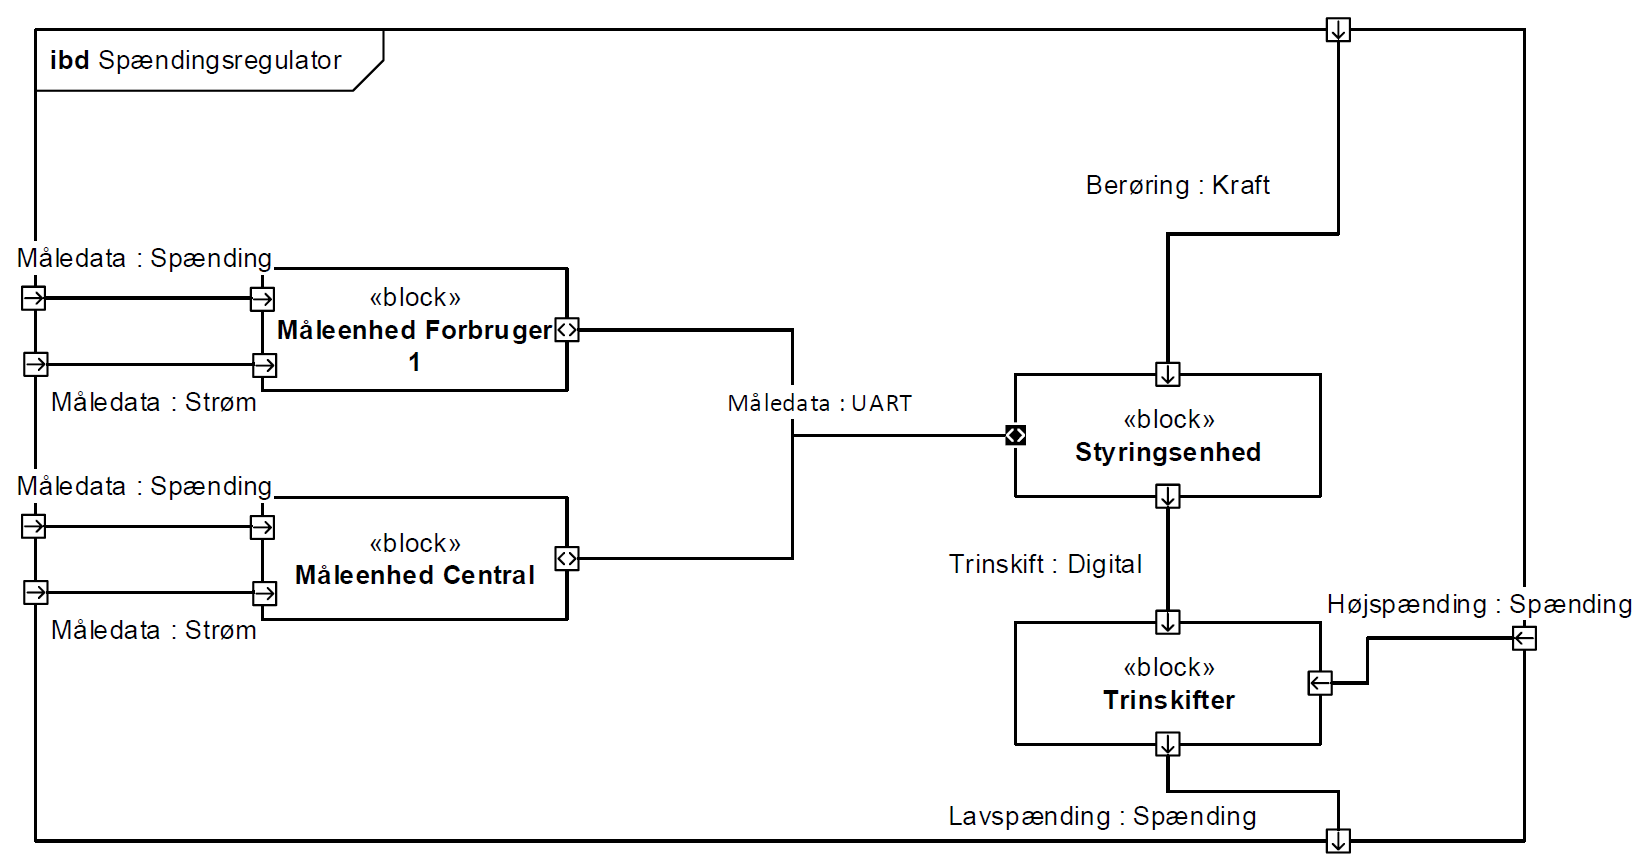
\includegraphics[width=0.8\textwidth]{Figure/IBDSpaendingsregulator1}
	\caption{IBD for Spændingsregulator}
	\label{fig:IBDSp}
\end{figure}

\begin{table}[H]
	\centering
	\begin{tabular}{|l|l|l|l|p{4cm}|}
		\hline
		\textbf{Blok} & \textbf{Navn} & \textbf{Type} & \textbf{Signal} & 
		\textbf{Beskrivelse} \\\hline
		
		\multirow{3}{*}{Måleenhed} 
		& Måledata & Spænding & In & Måledata er spændingsniveauet på distributionslinjen. \\\hhline{~----} 
		& Måledata & Strøm & In & Måledata er strømniveauet på distributionslinjen. \\\hhline{~----} 
		& Måledata & UART & InOut & UART forbindelse til Styringsenhed \\\hline
		
		\multirow{3}{*}{Styringsenhed} 
		& Måledata & UART & Inout & UART forbindelse til Måleenhed \\\hhline{~----} 
		& Berøring & Kraft & In & Tryk på Brugergrænseflade \\\hhline{~----} 
		& Trinskift & Digital & Out & Trinskift er en digital kommando til Trinskifter \\\hline
		
		\multirow{3}{*}{Trinskifter} 
		& Trinskift & Digital & In & Trinskift er en digital kommando fra Styringsenhed. \\\hhline{~----} 
		& Højspænding & Spænding & In & Er spændingen på højspændingssiden af tranformeren. \\\hhline{~----} 
		& Lavspænding & Spænding & Out & Er spændingen på lavspændingssiden af transformeren. \\\hline
	\end{tabular}
	\caption{Signalbeskrivelse for Spændingsregulator}
	\label{tab:SignalbeskrivelseSp}
	
\end{table}


\begin{figure}[htbp] % (alternativt [H])
	\centering
	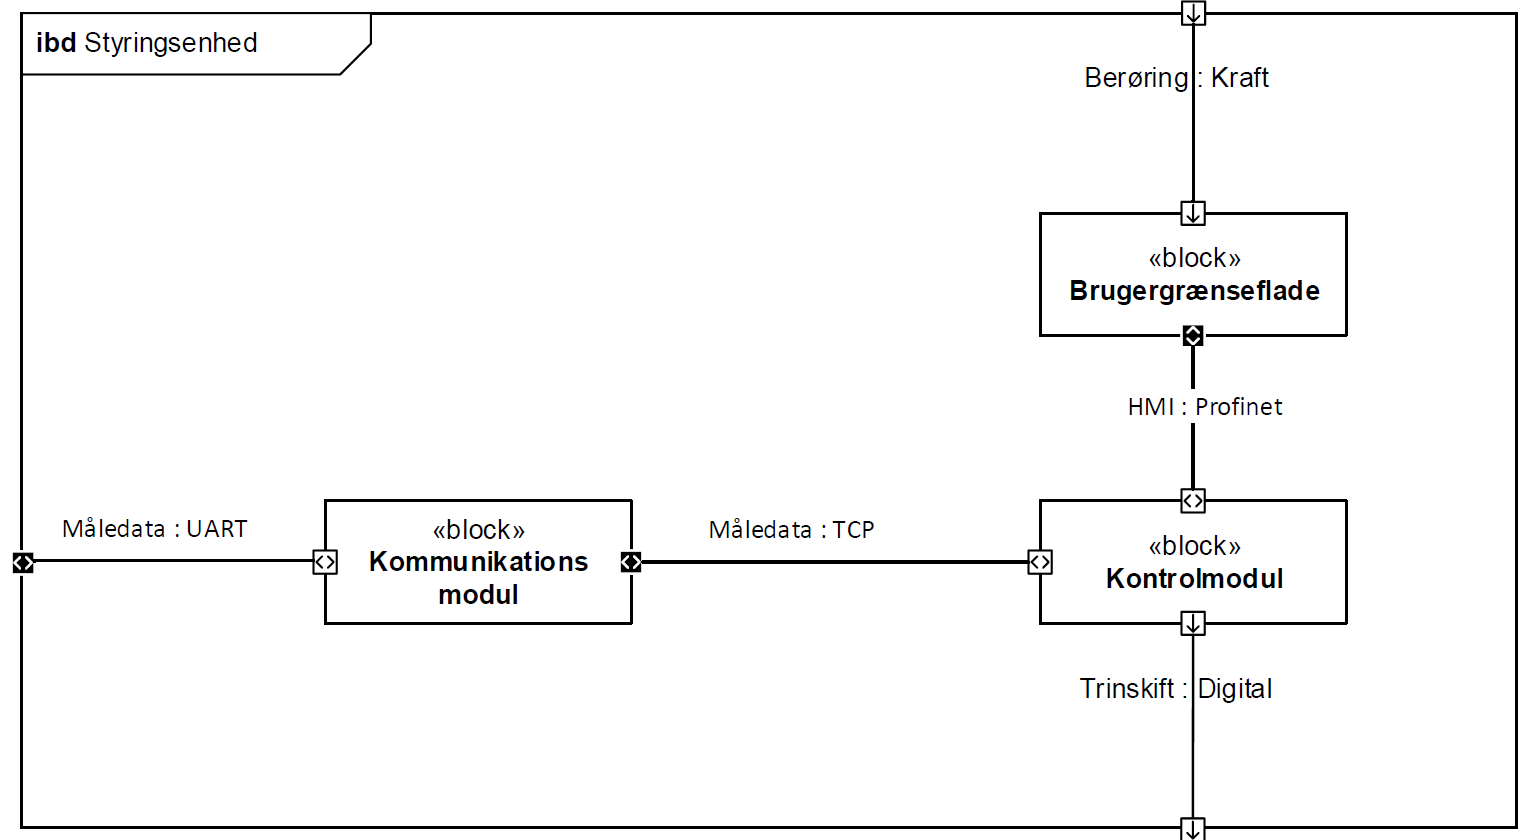
\includegraphics[width=0.8\textwidth]{Figure/IBDStyringsenhed1}
	\caption{IBD for Styringsenhed}
	\label{fig:IBDSt}
\end{figure}

\begin{table}[H]
	\centering
	\begin{tabular}{|l|l|l|l|p{4cm}|}
		\hline
		\textbf{Blok} & \textbf{Navn} & \textbf{Type} & \textbf{Signal} & 
		\textbf{Beskrivelse} \\\hline
		
		\multirow{2}{*}{Brugergrænseflade} 
		& Berøring & Kraft & In & Tryk på Brugergrænseflade \\\hhline{~----} 
		& HMI & Profinet & InOut & Forbindelse til Kontrolmodul \\\hline
		
		\multirow{3}{*}{Kontrolmodul} 
		& HMI & Profinet & InOut & Forbindelse til Brugergrænseflade \\\hhline{~----} 
		& Trinskift & Digital & Out & Trinskift er en digital kommando til Trinskifter \\\hhline{~----} 
		& Måledata & TCP & InOut & TCP forbindelse til Kommunikationsmodul \\\hline
		
		\multirow{2}{*}{Kommunikationsmodul} 
		& Måledata & TCP & InOut & TCP forbindelse til Kontrolmodul \\\hhline{~----} 
		& Måledata & UART & InOut & UART forbindelse til Måleenhed \\\hline
	\end{tabular}
	\caption{Signalbeskrivelse for Styringsenhed}
	\label{tab:SignalbeskrivelseSt}
	
\end{table}


\newpage
% !TEX root = ../../prj4projektdokumentation.tex
% SKAL STÅ I TOPPEN AF ALLE FILER FOR AT MASTER-filen KOMPILERES 

\section{Allokeringsdiagram}
På figur \ref{fig:Allokering} ses allokeringsdiagram for spændningsregulatoren. Diagrammet er lavet for at danne overblik over softwaren, derfor er analog moduler undladt. Styringsenheden laver et output til trin transformeren og Måleenehederne får input fra belastninger. Det er heller ikke vist på diagrammet. Diagrammet viser hvilke platforme de logiske blokke skal laves på, og hvordan kommunikationen er mellem blokkene

\begin{enumerate}
	\item Styringsenheden allokeres på en PLC
	\item Brugergrænsefladen allokeres på en HMI skærm
	\item Måleenhederne allokeres på PSoCs
\end{enumerate}   

\begin{figure}[htbp] % (alternativt [H])
	\centering
	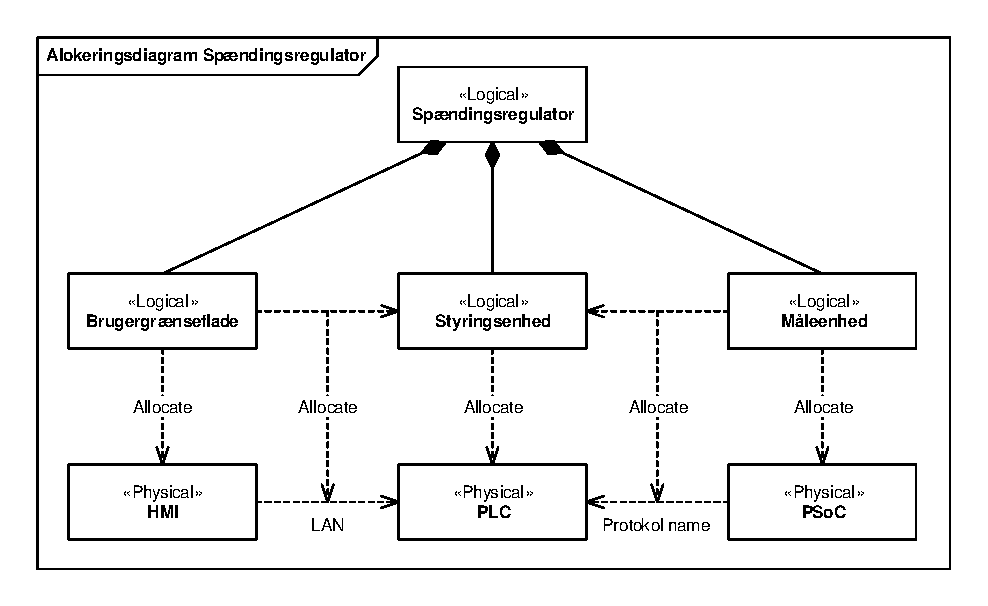
\includegraphics[width=0.9\textwidth]{Figure/Allokering}
	\caption{Allokeringsdiagram for spændingsregulator}
	\label{fig:Allokering}
\end{figure}
% !TEX root = ../prj4projektdokumentation.tex
% SKAL STÅ I TOPPEN AF ALLE FILER FOR AT MASTER-filen KOMPILERES 

\chapter{Foranalyse}

\section{Valg af transformer}
Emir udleverede to transformere. Den ene er der ingen mærkeplade og ledningerne var alle samme farve. Den anden har mærkeplade og forskellige farvet ledninger. De to transformere blev begge undersøgt i laboratoriet, med en 18VAC på primærside, derefter måltes spændingen på de forskellige trin. Transformeren uden mærkeplade hoppede små skridt fra ca 3 - 4.5V, hvor transformeren med mærkeplade havde skridt på 1 V fra 0 til 8V. Gruppen blev enige om at det var ligegyldigt om det var små eller store skridt transformeren hoppede, bare protypen blev lavet så den passede til transformeren. Det blev derfor besluttet at anvende transformeren med mærkeplade og forskellige farvet ledninger. 

\section{Valg af styringsenhed}
Det er besluttet at lave Styringsenheden på en PLC, dette gøres for at realisere, hvordan det ville laves i virkeligheden. Alternativt kunne det laves på en PSOC eller Arduino, men da der på dette semester er undervisning i PLC styring virker det derfor oplagt.

\section{Overvejelser omkring måleenhederne}
Det var først tænkt at der kunne laves eller købes nogle sensorer som skulle tilsluttes PLC'en. PLC'en kan dog ikke måle hurtigt nok på AC forbindelser til at få et reelt billed af signalet. Derfor bruges PSOC til at måle og sample signalet og sende det derfra til PLC'en.

\section{Protokoller}




\printbibliography

\end{document}


